% ------------------------------------------------------------------------
% -*-TeX-*- -*-Hard-*- Smart Wrapping
% ------------------------------------------------------------------------

% REF\_1 - http://neuralnetworksanddeeplearning.com/chap1.html

% REF\_2 - Large-Scale Machine Learning with Stochastic Gradient Descent Leon Bottou

% REF\_3 - Chin-Wei Hsu, Chih-Chung Chang and Chih-Jen Lin (2010). A practical guide to support vector classification. Technical Report, National Taiwan University.


\def\baselinestretch{1}

\chapter{Experimentation and Discussion}

%%% ----------------------------------------------------------------------

% intro text here

\smallskip

%%% ----------------------------------------------------------------------
\goodbreak

\section{Evaluating the Counting-by-Regression Approach}
\subsection{Evaluation Methodology}
%describe ways used to evaluate - https://en.wikipedia.org/wiki/Regression_validation

\subsection{System Performance}
%experiments and results and discuss

\section{Evaluating the Counting-by-Detection Approach}
\subsection{The Model Setup}
The model used for the prediction (and in essence, detection) of grains was the artificial neural network using the Multi-Layer Perceptron (MLP) learning algorithm. The MLP made use of the \textit{\textbf{sigmoid function $\sigma$}} (also known as the \textbf{\textit{logistic function}}) as its activation function (REF\_1). The sigmoid function is as follows:
\begin{equation}
\sigma(x) = \frac{1}{1 + e^{-x}}
\end{equation}
The MLP used the \textit{\textbf{stochastic gradient descent}} algorithm for tuning its weights (REF\_2). Neural network possess a number of \textit{hyperparameters} which cannot be learned by fitting the model to the data but could influence their performance greatly. In particular, the MLP neural network used for this task had the following hyperparameters:
\begin{itemize}
\item \textit{hidden layer arrangement} - This refers to the number of hidden layers in the network as well as the number of neurons in each layer.
\item \textit{alpha} - This is the \textit{L2} regularization penalty for minimizing prediction error
\item \textit{learning rate} - This controls how quickly the gradient descent algorithm travels down the slope to find the minimum of the cost function when tuning the weights of the neurons.
\item \textit{batch size} - This refers to the size of the mini-batches chosen by the stochastic gradient descent algorithm to speed up the learning process
\end{itemize}
In order to get the best performance from the MLP, an attempt was made to determine the optimum values for these hyperparameters. To do this, the \textit{\textbf{Grid Search}} algorithm for hyperparameter optimization was employed. Grid search is simply an exhaustive search through a manually specified subset of the hyperparameter space (REF\_3).

\subsection{Evaluation Methodology}
350 images were hand selected and labeled to form a data set. The images were selected in a balanced manner with roughly the same amount of instances of all classes. All of this data was used for training and building the neural network. The same data was also used in evaluating the performance of the neural network. Things were done this way because while there was no shortage of sub-images, they had to be labeled manually. Labeling more sub-images for testing than the 350 images already labeled would have been a time-consuming process. On the other hand, we thought it would have been unwise to split the data into separate training and testing sets as the dataset was not very large to begin with. To overcome this problem, \textit{cross validation} was used for evaluation.\\ \\
%
Cross validation aims to define a dataset to ``test'' a model in the training phase, in order to limit problems like overfitting and give an idea of how the model will generalize to an independent dataset. For evaluating the accuracy of our MLP classifier, 5-fold cross validation was used. The data was split into five sets and five iterations of the following procedure were carried out. At each iteration, one set was selected to be the training set (used to build the classifier) and the remaining four were used to test the classifier. The set selected as the training set was changed at each of the five iterations. Once all the iterations were completed, the accuracies from each one was averaged to give the mean accuracy of the classifier. This was needed to get as good a classifier as possible. This is because MLP neural networks start with random weights assigned to the neurons. The values of these starting weights affect the weights that the MLP ends up with, thereby affecting its performance. To get the best model possible, the neural network was built (with random weights) $n$ times. After each build, it was evaluated using the 5-fold cross validation strategy to paint a picture of its accuracy. The MLP with the best accuracy (found to be $81.12\%$) was selected and serialized to disk to be used as the model as needed.


\bigskip

%%% ----------------------------------------------------------------------
\goodbreak

\subsection{System Performance}
\begin{table}[hp!]
  \centering
  \begin{tabular}{ | c | c | c | c |}
    \hline
    Image & Actual count & Predicted count & Time taken \\ \hline
    \begin{minipage}{.3\textwidth}
      \begin{center}
		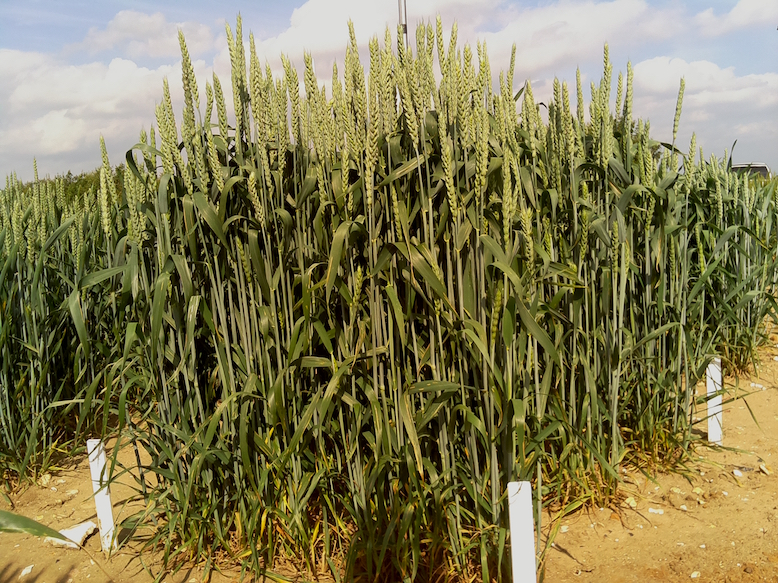
\includegraphics[width=\linewidth]{Images/001}
      \end{center}
    \end{minipage}
    &
    %\begin{minipage}[t]{5cm}
      xxx
    %\end{minipage}
    & 
    %\begin{minipage}{5cm}
      1435
    %\end{minipage}
    & 
    %\begin{minipage}{5cm}
      215
    %\end{minipage}
    \\ \hline
    %%% NEW LINE %%%
    \begin{minipage}{.3\textwidth}
      \begin{center}
		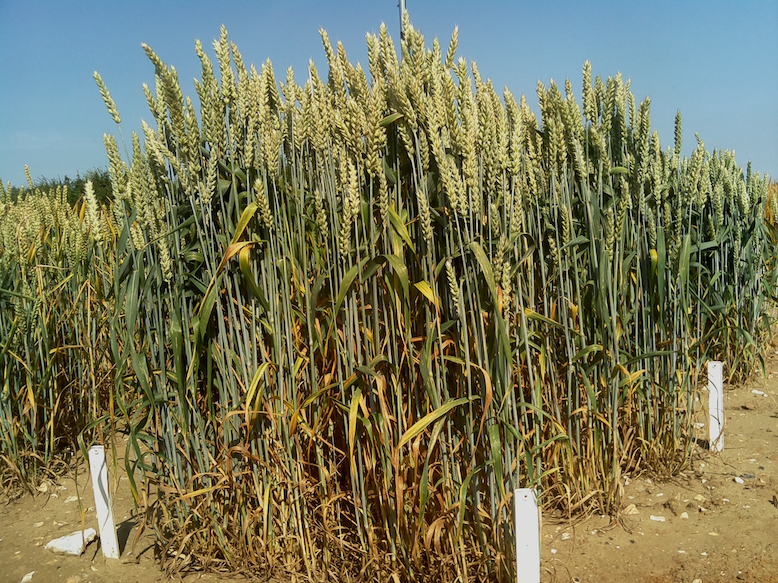
\includegraphics[width=\linewidth]{Images/002}
      \end{center}
    \end{minipage}
    &
    %\begin{minipage}[t]{5cm}
      xxx
    %\end{minipage}
    & 
    %\begin{minipage}{5cm}
      yyy
    %\end{minipage}
    & 
    %\begin{minipage}{5cm}
      zzz
    %\end{minipage}
    \\ \hline
    %%% NEW LINE %%%
    \begin{minipage}{.3\textwidth}
      \begin{center}
		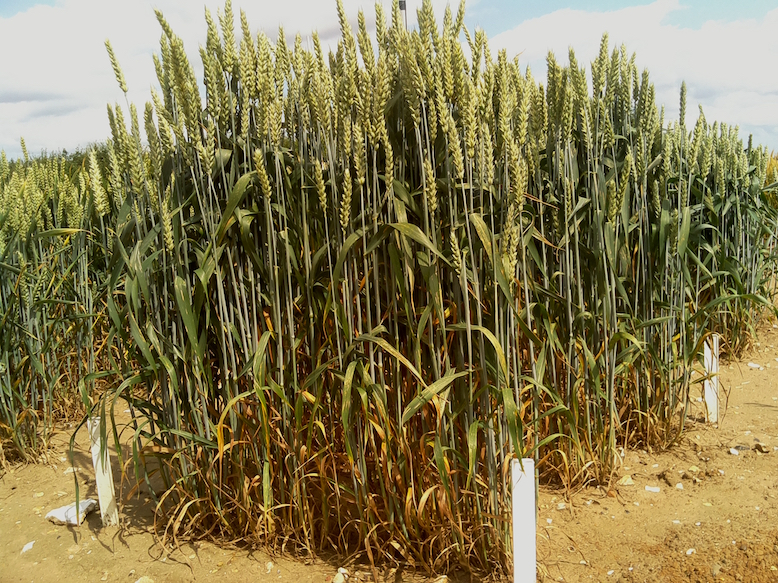
\includegraphics[width=\linewidth]{Images/003}
      \end{center}
    \end{minipage}
    &
    %\begin{minipage}[t]{5cm}
      xxx
    %\end{minipage}
    & 
    %\begin{minipage}{5cm}
      yyy
    %\end{minipage}
    & 
    %\begin{minipage}{5cm}
      zzz
    %\end{minipage}
    \\ \hline
    %%% NEW LINE %%%
    \begin{minipage}{.3\textwidth}
      \begin{center}
		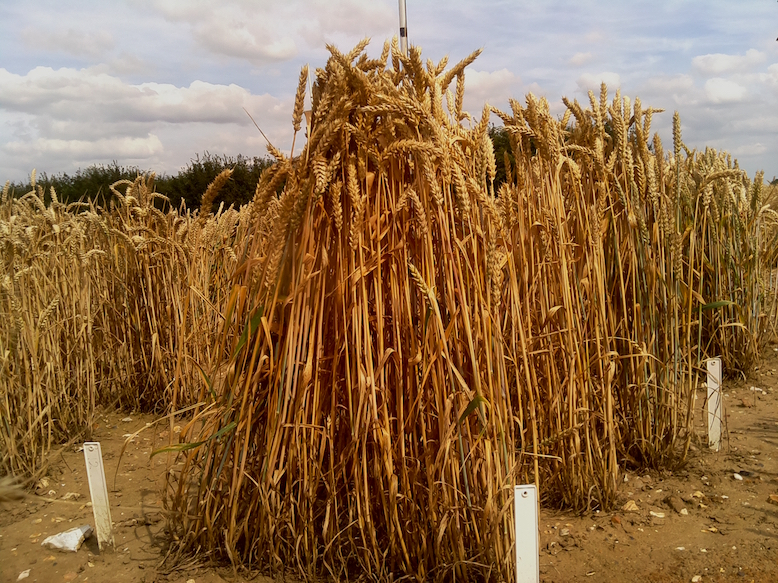
\includegraphics[width=\linewidth]{Images/004}
      \end{center}
    \end{minipage}
    &
    %\begin{minipage}[t]{5cm}
      xxx
    %\end{minipage}
    & 
    %\begin{minipage}{5cm}
      yyy
    %\end{minipage}
    & 
    %\begin{minipage}{5cm}
      zzz
    %\end{minipage}
    \\ \hline
    %%% NEW LINE %%%
    \begin{minipage}{.3\textwidth}
      \begin{center}
		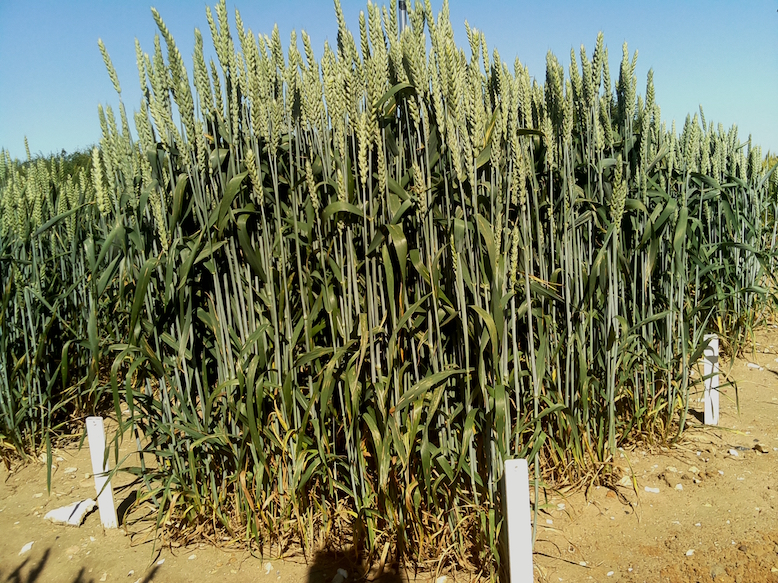
\includegraphics[width=\linewidth]{Images/005}
      \end{center}
    \end{minipage}
    &
    %\begin{minipage}[t]{5cm}
      xxx
    %\end{minipage}
    & 
    %\begin{minipage}{5cm}
      yyy
    %\end{minipage}
    & 
    %\begin{minipage}{5cm}
      zzz
    %\end{minipage}
    \\ \hline
    %%% NEW LINE %%%
    \begin{minipage}{.3\textwidth}
      \begin{center}
		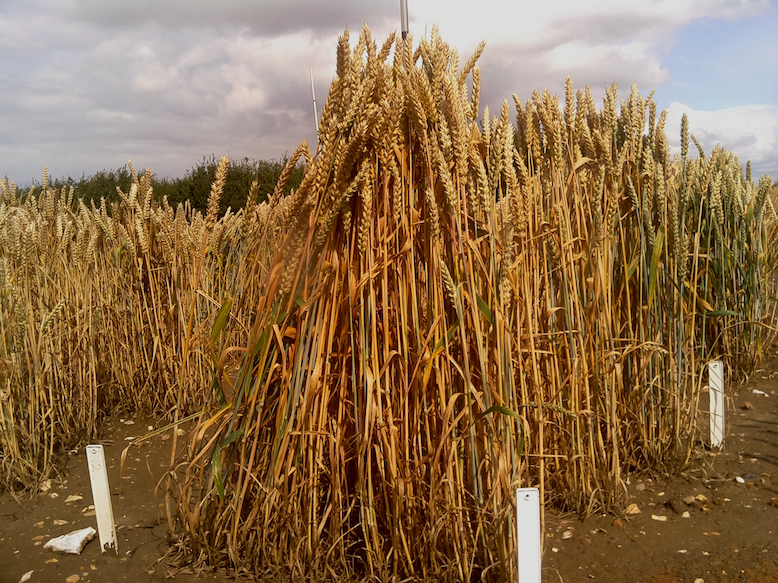
\includegraphics[width=\linewidth]{Images/006}
      \end{center}
    \end{minipage}
    &
    %\begin{minipage}[t]{5cm}
      xxx
    %\end{minipage}
    & 
    %\begin{minipage}{5cm}
      yyy
    %\end{minipage}
    & 
    %\begin{minipage}{5cm}
      zzz
    %\end{minipage}
    \\ \hline
  \end{tabular}
  \caption{Results of proposed system}\label{tbl:myLboro}
\end{table}

%%%%%%%%%%%%%%%%%%%%%%%%%%%%%%%%%%%%%%%%%%%%%%%%%%%%%%%%%%%%%
%%%% table pt 2 
%%%%%%%%%%%%%%%%%%%%%%%%%%%%%%%%%%%%%%%%%%%%%%%%%%%%%%%%%%%%%

\begin{table}[ht!]
  \centering
  \begin{tabular}{ | c | c | c | c |}
    \hline
    Image & Actual count & Predicted count & Time taken \\ \hline
    \begin{minipage}{.3\textwidth}
      \begin{center}
		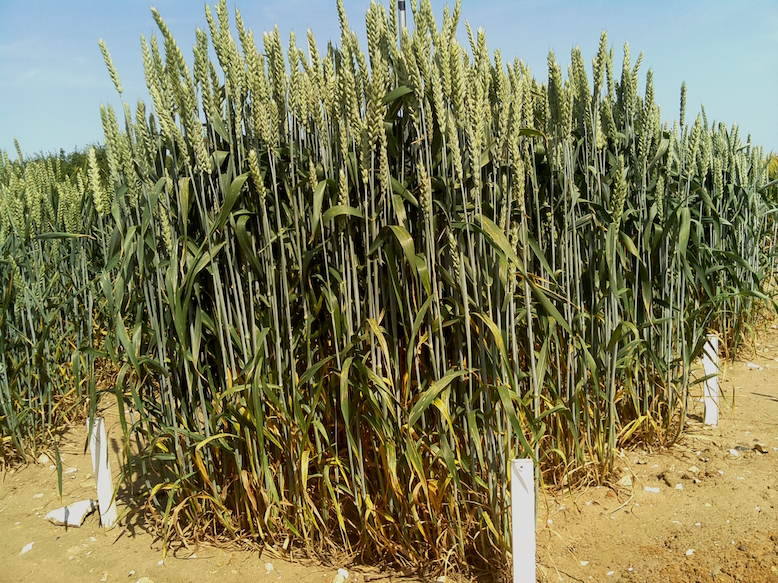
\includegraphics[width=\linewidth]{Images/008}
      \end{center}
    \end{minipage}
    &
    %\begin{minipage}[t]{5cm}
      xxx
    %\end{minipage}
    & 
    %\begin{minipage}{5cm}
      yyy
    %\end{minipage}
    & 
    %\begin{minipage}{5cm}
      zzz
    %\end{minipage}
    \\ \hline
    %%% NEW LINE %%%
    \begin{minipage}{.3\textwidth}
      \begin{center}
		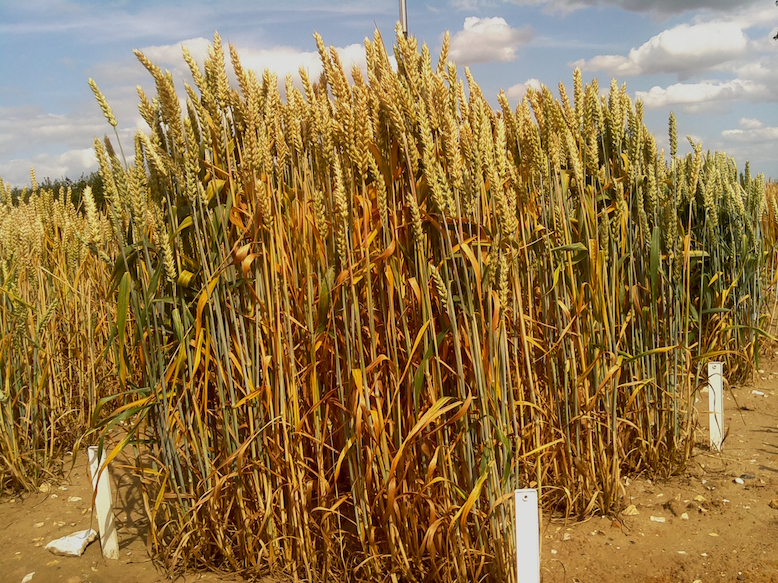
\includegraphics[width=\linewidth]{Images/009}
      \end{center}
    \end{minipage}
    &
    %\begin{minipage}[t]{5cm}
      xxx
    %\end{minipage}
    & 
    %\begin{minipage}{5cm}
      yyy
    %\end{minipage}
    & 
    %\begin{minipage}{5cm}
      zzz
    %\end{minipage}
    \\ \hline
    %%% NEW LINE %%%
    \begin{minipage}{.3\textwidth}
      \begin{center}
		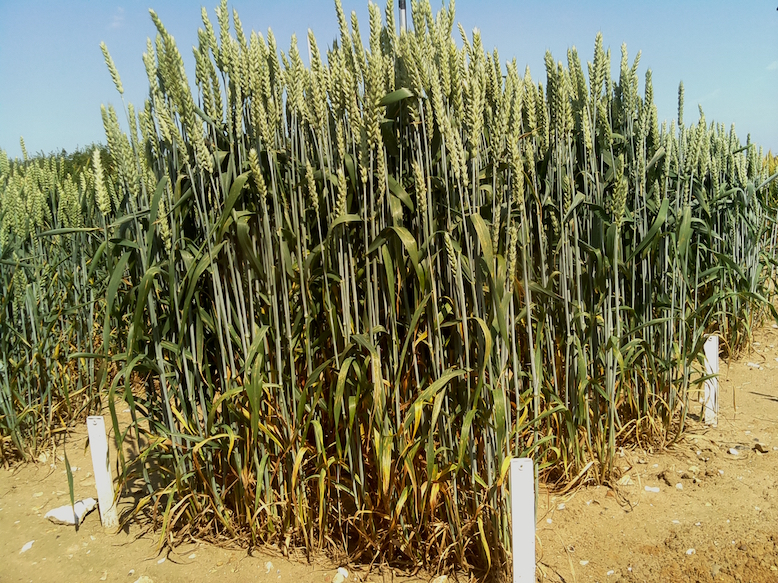
\includegraphics[width=\linewidth]{Images/010}
      \end{center}
    \end{minipage}
    &
    %\begin{minipage}[t]{5cm}
      xxx
    %\end{minipage}
    & 
    %\begin{minipage}{5cm}
      yyy
    %\end{minipage}
    & 
    %\begin{minipage}{5cm}
      zzz
    %\end{minipage}
    \\ \hline
    %%% NEW LINE %%%
    \begin{minipage}{.3\textwidth}
      \begin{center}
		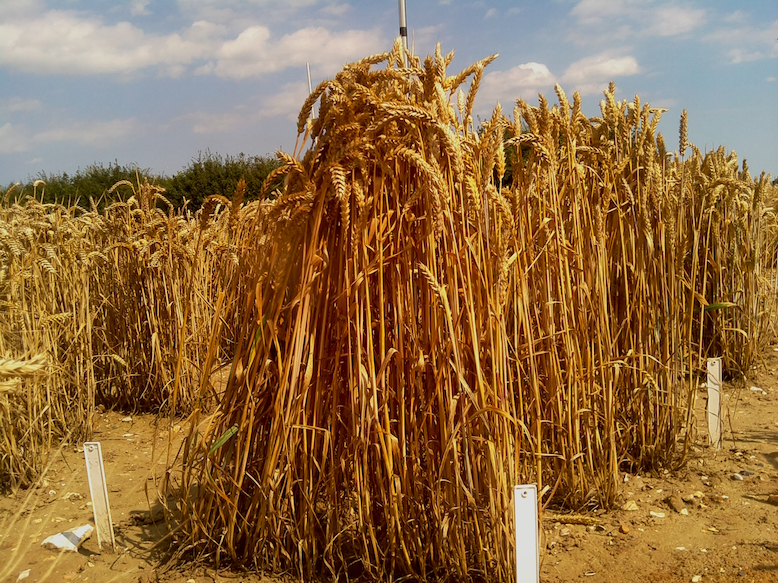
\includegraphics[width=\linewidth]{Images/011}
      \end{center}
    \end{minipage}
    &
    %\begin{minipage}[t]{5cm}
      xxx
    %\end{minipage}
    & 
    %\begin{minipage}{5cm}
      yyy
    %\end{minipage}
    & 
    %\begin{minipage}{5cm}
      zzz
    %\end{minipage}
    \\ \hline
    %%% NEW LINE %%%
    \begin{minipage}{.3\textwidth}
      \begin{center}
		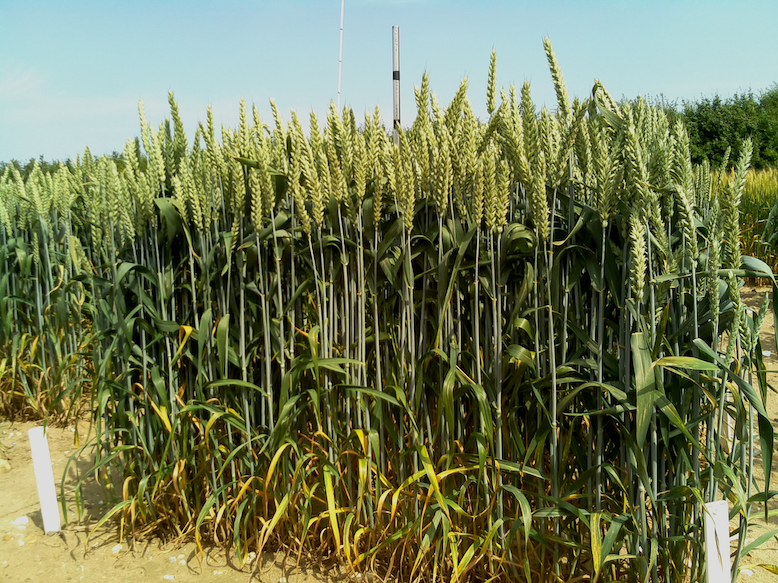
\includegraphics[width=\linewidth]{Images/012}
      \end{center}
    \end{minipage}
    &
    %\begin{minipage}[t]{5cm}
      xxx
    %\end{minipage}
    & 
    %\begin{minipage}{5cm}
      yyy
    %\end{minipage}
    & 
    %\begin{minipage}{5cm}
      zzz
    %\end{minipage}
    \\ \hline
    %%% NEW LINE %%%
  \end{tabular}
  \caption{Results of proposed system}\label{tbl:myLboro}
\end{table}
Having determined that the MLP could detect grains in images with an accuracy of $81.12\%$, it would be interesting to find out what this meant for the counting system itself. Tables 5.1 and 5.2 show the actual and predicted counts for the images provided as well as the time taken for the system to compute the counts. From these tables, it can be seen that the system seemed to perform better on some images than others. This was due to the fact that in the ROI extraction stage, the clusters to be extracted from the original image were hardcoded. This caused problems because the hardcoded clusters were not always the optimum (or sometimes even particularly good) clusters to select as regions of interest. A way around this problem would be to manually select the clusters denoting regions of interest to be extracted before before passing a query image to the system. A simple interactive program was built to this end. FIG\_ shows a screenshot of the ROI extraction interface. The program allows a user to upload an image and set the number of clusters that they wish to detect using the k-means clustering algorithm. The program then displays the image with the clusters overlayed over it and the user is able to select the clusters that they would like to extract. While this method might be slightly labour-intensive when a medium to large number of images need to have their grains counted, it yields much better performance. The trade-off here between labour-intensiveness and performance is something that would need to be considered in practice.
\begin{figure}[ht!]
\centering
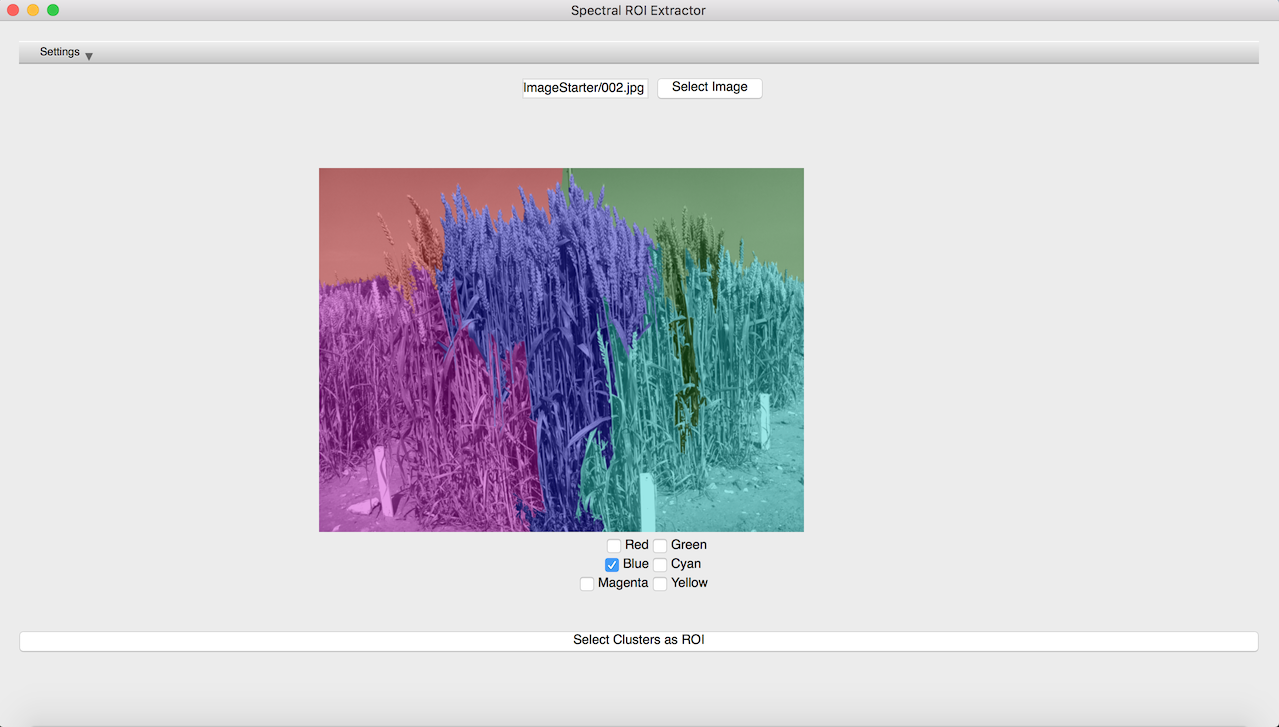
\includegraphics[scale=0.7]{Images/gui}
\caption{Interactive program for manual ROI extraction}
\label{fig1}
\end{figure}

\bigskip

%%% ----------------------------------------------------------------------
\goodbreak

\section{Comparisons}
It was difficult to properly evaluate the counting-by-detection approach. While it showed poorer results by being off the actual count by more than the counting-by-detection method, it should be noted that it was trained on only 7 wheat images and tested on the remaining 6. Using only 7 images would definitely not have built a very good model. The counting-by-detection approach on the other hand had access to 5000 potential examples from each wheat image. Therefore, while the counting-by-detection approach out-performed the counting-by-regression approach, it is still too soon to write off the regression approach as being inferior. However, because we know the accuracy of regression approaches is limited as there is no universal function that can map images to grain counts for any and all images. If a system can correctly detect grains in images (of any kind) to a reasonable extent, such a system would outclass any built on regression approaches\\ \\
%
The system proposed relies on a machine learning classifier for grain detection. Our solution makes use of a neural network. We tried other classifiers to see how they all measured up. For image classification, neural networks and support vector machines perform best so the two were pit against each other in order to determine which was best for this problem. In particular, an MLP neural network and an SVM with the \textit{radial basis function} as the kernel function were used. While the SVM was hundreds of times faster than the neural network, it only yielded a prediction accuracy of $65.9\%$ while the neural network yielded an accuracy of $81.12\%$. Despite the fact that the SVM was able to count grains in a fraction of the time that the neural network did, the difference in prediction accuracy was too great to be disregarded in favour of speed. There are still more kinds of neural networks besides the MLP variation used in our solution and in the future, we intend to look into how they can be applied to the problem. Convolutional neural networks are one such example. 



\bigskip

%%% ----------------------------------------------------------------------



